% Provenance (never printed): old premiere S material on magmatic rocks (volcanic
% and plutonic textures and cooling rate; basalt/gabbro, andesite/diorite,
% rhyolite/granite; order of crystallisation, told). Cooling of sheets from
% figdata/grade-11/dyke_cooling.py (Delaney 1986 parameters; kappa from England
% et al. 2007). Fractional crystallisation is Year 2's; metamorphism (contact
% aureoles) is g12.03's: not developed here.
\chapter{Les roches magmatiques}\label{ch:g11:igneous-rocks}

Sur la côte nord de l'Irlande, des colonnes de pierre serrées les unes
contre les autres descendent en gradins dans la mer~: la Chaussée des
Géants, un basalte qui a refroidi à partir d'une lave. Dans le parc de
Yosemite, en Californie, la paroi de granite d'El Capitan s'élève à quelque
\qty{900}{m} au-dessus du fond de la vallée, un seul massif de roche à gros
grains. Tous deux ont cristallisé à partir d'un magma. Le basalte a refroidi
en surface, ses cristaux trop petits pour être vus~; le granite a refroidi
profondément sous terre, ses cristaux assez grands pour être vus, et on ne
le voit aujourd'hui que parce que les roches qui le recouvraient ont été
usées. Ce chapitre lit dans les grains d'une roche à quelle vitesse, et à
quelle profondeur, elle a refroidi.
% ledger: photo:g11-giants-causeway, photo:g11-el-capitan, tulane:intrusions

\begin{omfigure}
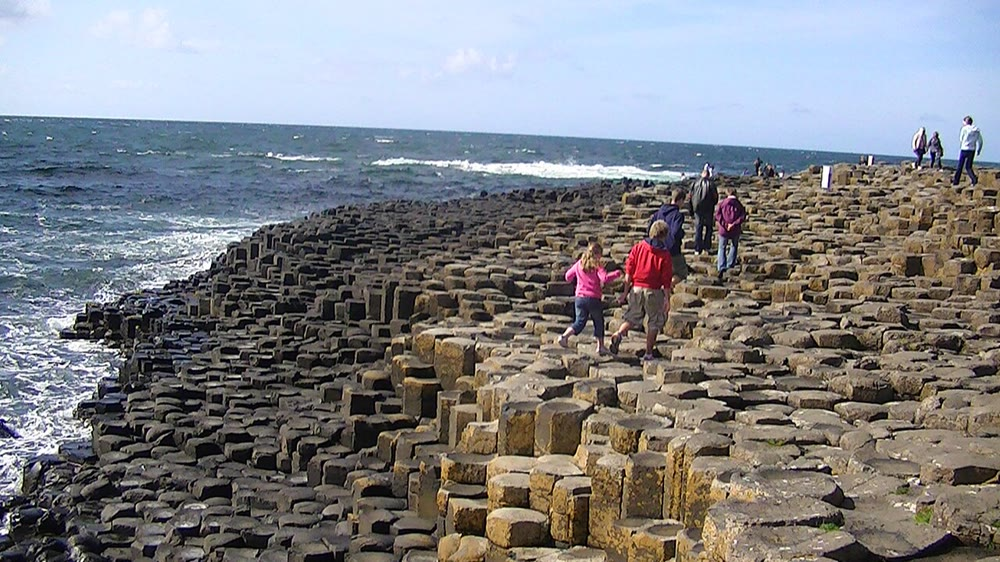
\includegraphics[height=4.3cm]{images/book2/g11-bishop-giants-causeway.jpg}\hspace{0.04\linewidth}%
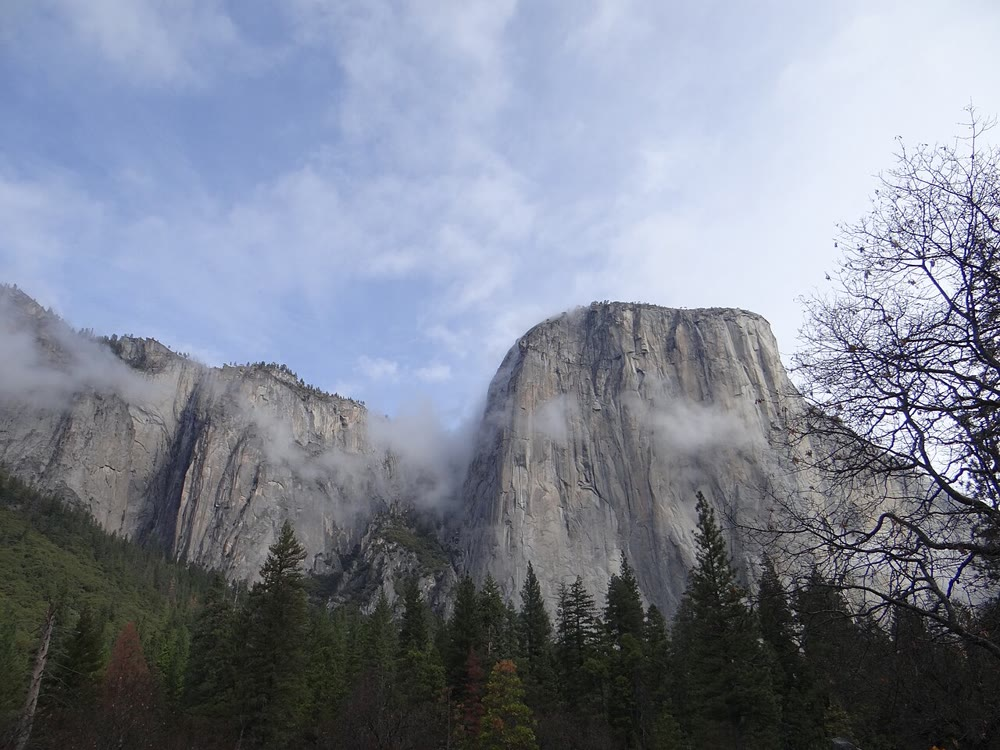
\includegraphics[height=4.3cm]{images/book2/g11-usgs-el-capitan.jpg}

{\small À gauche~: colonnes de basalte de la Chaussée des Géants, en Irlande
du Nord. Photographie Adam Bishop (CC~BY-SA~3.0). À droite~: El Capitan, à
Yosemite, en Californie, une paroi de granite haute d'environ \qty{900}{m}.
Photographie U.S. Geological Survey (CC0).}
\end{omfigure}
% ledger: photo:g11-giants-causeway, photo:g11-el-capitan

\begin{recall}
Le magma est de la roche fondue sous la surface~; il fait éruption sous
forme de lave, calmement ou de façon explosive (livre~1, année~7). Une
roche magmatique (ou ignée) est une roche formée quand de la roche fondue
refroidit et devient solide (livre~1, année~6). Le basalte est une \omterm{def:g11:igneous-rocks:volcanic-plutonic}{roche
volcanique} sombre, le granite une roche claire faite de feldspath, de quartz
et de mica (livre~1, année~6). La \omterm{def:g11:ocean-ridges:peridotite}{péridotite} du manteau fond partiellement
en remontant sous une dorsale, ce qui donne le basalte et le \omterm{def:g11:ocean-ridges:gabbro}{gabbro} de la
\omterm{def:g11:ocean-ridges:oceanic-lithosphere}{croûte océanique} (\cref{ch:g11:ocean-ridges}). Les \omterm{def:g11:minerals:rock-forming}{silicates constitutifs
des roches} sont l'olivine, les pyroxènes, les amphiboles, les micas, les
feldspaths et le quartz~; les feldspaths sont le feldspath potassique et le
plagioclase, une série allant du pôle riche en calcium au pôle riche en
sodium (\cref{ch:g11:minerals}). La chaleur se propage par conduction sur
une distance d'environ $\sqrt{\kappa t}$ en un temps $t$, où $\kappa$ est
la diffusivité thermique (\cref{ch:g11:subduction-zones}).
\end{recall}
% ledger: tulane:ridge-rocks, england:kelvin

\section{Roches volcaniques et roches plutoniques}

\begin{definition}[Roche volcanique~; roche plutonique]\label{def:g11:igneous-rocks:volcanic-plutonic}
Une roche magmatique, formée par la cristallisation d'un magma, est
\emph{volcanique}\index{roche volcanique}
(ou effusive) quand le magma s'est solidifié à la surface de la Terre, sous
forme de lave, et \emph{plutonique}\index{roche plutonique} (ou intrusive)
quand il a cristallisé en profondeur, à l'intérieur d'autres roches.
\end{definition}
% ledger: tulane:magma-types

La différence se voit à la taille des cristaux. Un cristal grandit en
ajoutant des atomes pris au liquide qui l'entoure, et cela demande du temps.
En surface, une lave perd vite sa chaleur dans l'air ou dans l'eau~: les
matériaux projetés dans l'air ou dans l'eau refroidissent en quelques
secondes, une coulée de lave en quelques jours à quelques semaines. En
profondeur, les roches encaissantes sont chaudes et le magma perd sa chaleur
lentement~: une \omterm{def:g11:igneous-rocks:intrusion}{intrusion} peu profonde refroidit en quelques mois à quelques
années, une grande \omterm{def:g11:igneous-rocks:intrusion}{intrusion} profonde peut demander des millions d'années.
Un refroidissement rapide donne de nombreux petits cristaux, ou pas de
cristaux du tout~; un refroidissement lent en donne moins, mais bien plus
grands.
% ledger: tulane:cooling-times, tulane:textures

\begin{definition}[Texture]\label{def:g11:igneous-rocks:texture}
La \emph{texture}\index{texture (d'une roche)} d'une roche est la taille, la
forme et l'agencement de ses grains. Une roche magmatique est
\emph{vitreuse} quand elle n'a pas de cristaux, \emph{à grain fin} quand ses
cristaux sont trop petits pour être distingués à l'œil nu, et \emph{à gros
grains} quand on peut tous les voir.
\end{definition}
% ledger: tulane:textures

Une lave trempée avant qu'aucun cristal ait pu grandir devient un verre~:
l'obsidienne, noire et vitreuse, se casse avec la cassure conchoïdale d'une
bouteille. Le basalte est à grain fin~: à la main, on ne peut pas identifier
ses minéraux, et même en \omterm{def:g11:minerals:thin-section}{lame mince} ses cristaux sont petits (le basalte du
\cref{ch:g11:minerals}). Le granite, le \omterm{def:g11:ocean-ridges:gabbro}{gabbro} et la \omterm{def:g11:igneous-rocks:rock-names}{diorite} sont à gros
grains~: chaque grain se voit.
% ledger: photo:g11-obsidian, photo:g11-basalt, tulane:textures

\begin{definition}[Phénocristal~; porphyrique]\label{def:g11:igneous-rocks:porphyritic}
Un \emph{phénocristal}\index{phenocristal@phénocristal} est un grand cristal
pris dans une masse de cristaux bien plus petits ou de verre, la
\emph{pâte}. Une roche à phénocristaux est
\emph{porphyrique}\index{porphyrique}.
\end{definition}
% ledger: tulane:textures

Une \omterm{def:g11:igneous-rocks:texture}{texture} \omterm{def:g11:igneous-rocks:porphyritic}{porphyrique} enregistre deux étapes de refroidissement~: d'abord
lente, en profondeur, pendant que les \omterm{def:g11:igneous-rocks:porphyritic}{phénocristaux} grandissaient dans un
magma encore surtout liquide~; puis rapide, quand le magma est monté et a
fait éruption, ou a été injecté dans une roche froide, et que le reste du
liquide s'est figé en pâte.
% ledger: tulane:textures

\begin{omfigure}
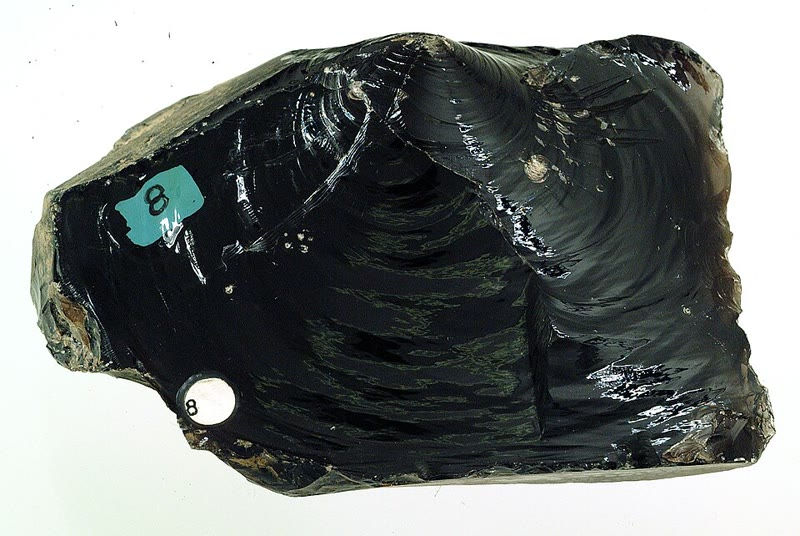
\includegraphics[height=2.75cm]{images/book2/g11-geodil-obsidian.jpg}\hfill
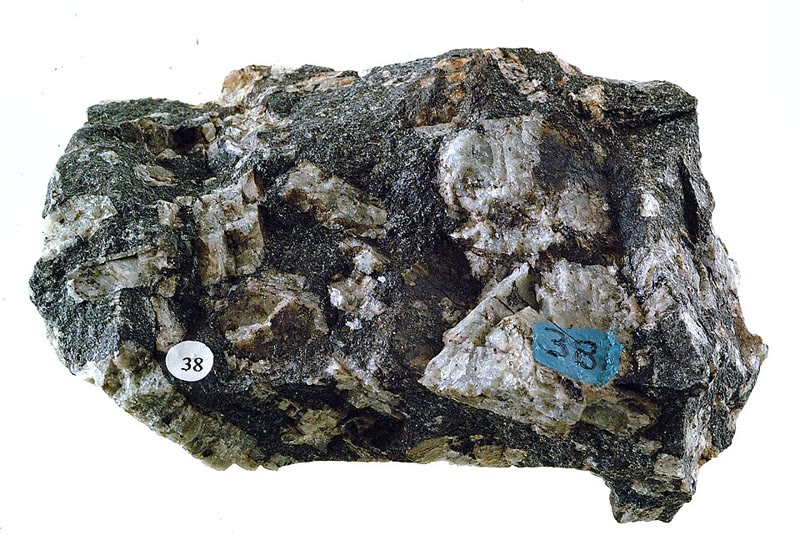
\includegraphics[height=2.75cm]{images/book2/g11-geodil-diabase-porphyry.jpg}\hfill
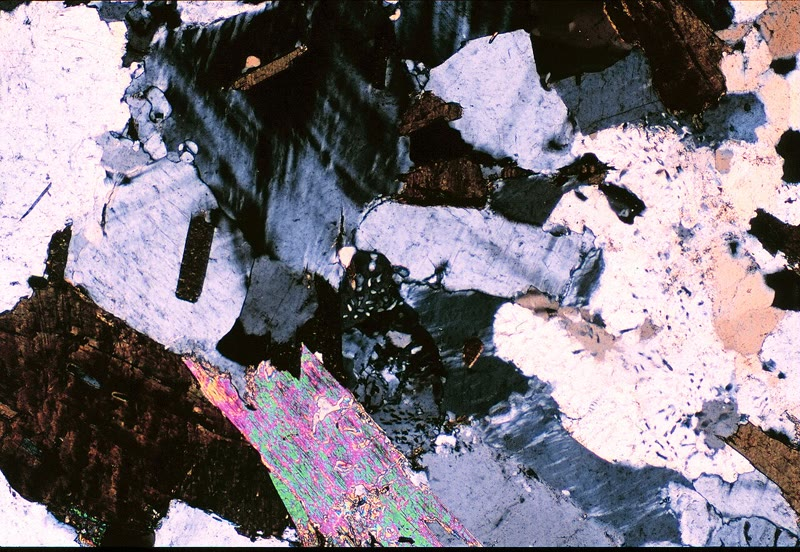
\includegraphics[height=2.75cm]{images/book2/g11-geodil-granite-xpl.jpg}\hfill
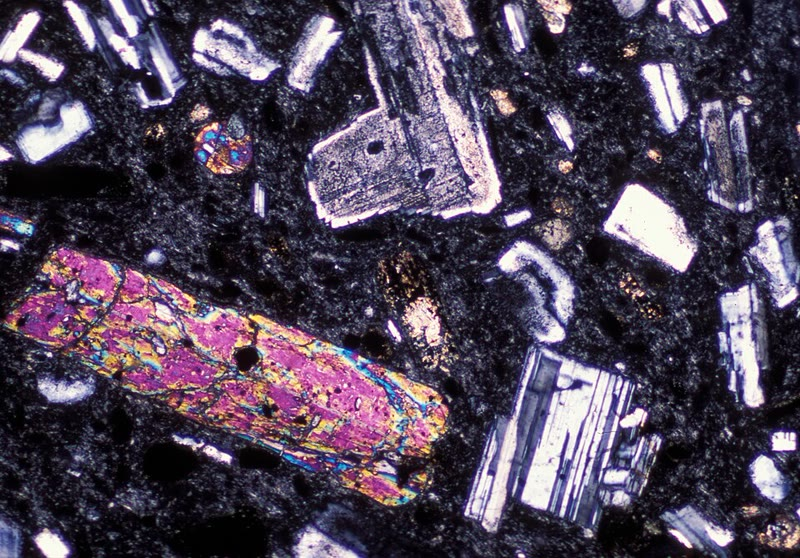
\includegraphics[height=2.75cm]{images/book2/g11-geodil-andesite-xpl.jpg}

{\small De gauche à droite~: une obsidienne, un verre \omterm{def:g11:igneous-rocks:volcanic-plutonic}{volcanique}, avec sa
cassure courbe conchoïdale (\qty{9.5}{cm} de large)~; une roche
\omterm{def:g11:igneous-rocks:porphyritic}{porphyrique}, avec des \omterm{def:g11:igneous-rocks:porphyritic}{phénocristaux} trapus de plagioclase dans une pâte plus
fine (\qty{9}{cm})~; puis deux \omterm{def:g11:minerals:thin-section}{lames minces} entre polariseurs croisés~: un
granite, aux grains tous grands et imbriqués --- biotite brune, muscovite
aux couleurs vives, plagioclase rayé, quartz gris et blanc~; une \omterm{def:g11:igneous-rocks:rock-names}{andésite},
avec des \omterm{def:g11:igneous-rocks:porphyritic}{phénocristaux} de plagioclase et d'amphibole dans une pâte à grain
fin. Photographies Twyla Baker, Mike Davis et Darla Sondrol, Geology
Digital Image Library (CC0).}
\end{omfigure}
% ledger: photo:g11-obsidian, photo:g11-diabase-porphyry, photo:g11-granite-xpl, photo:g11-andesite-xpl

\section{Nommer les roches magmatiques}

La seconde clé d'une roche magmatique est sa chimie, et surtout sa teneur
en silice, \ce{SiO2}, qui va dans les magmas courants d'environ
\qty{45}{\percent} à environ \qty{75}{\percent} de la masse.

\begin{definition}[Mafique~; intermédiaire~; felsique]\label{def:g11:igneous-rocks:felsic-mafic}
Un magma, ou la roche qu'il forme, est \emph{mafique}\index{mafique} quand
il contient environ \qty{45}{\percent} à \qty{55}{\percent} de \ce{SiO2} et
qu'il est riche en fer, en magnésium et en calcium~;
\emph{intermédiaire}\index{intermediaire (roche)@intermédiaire (roche)}
entre \qty{55}{\percent} et \qty{65}{\percent}~;
\emph{felsique}\index{felsique} quand il contient environ
\qty{65}{\percent} à \qty{75}{\percent} de \ce{SiO2} et qu'il est pauvre en
fer, en magnésium et en calcium mais riche en sodium et en potassium.
\end{definition}
% ledger: tulane:magma-types, earle:magma-oxides

Chaque type de magma donne deux roches de même chimie, l'une \omterm{def:g11:igneous-rocks:volcanic-plutonic}{volcanique} et
à grain fin, l'autre \omterm{def:g11:igneous-rocks:volcanic-plutonic}{plutonique} et à gros grains. Le basalte et le \omterm{def:g11:ocean-ridges:gabbro}{gabbro}
forment la paire \omterm{def:g11:igneous-rocks:felsic-mafic}{mafique}, rencontrée avec la \omterm{def:g11:ocean-ridges:oceanic-lithosphere}{croûte océanique}~; le granite
est la \omterm{def:g11:igneous-rocks:volcanic-plutonic}{roche plutonique} \omterm{def:g11:igneous-rocks:felsic-mafic}{felsique}. Trois noms complètent l'ensemble.

\begin{definition}[Andésite~; diorite~; rhyolite]\label{def:g11:igneous-rocks:rock-names}
L'\emph{andésite}\index{andesite@andésite} et la
\emph{diorite}\index{diorite} sont la \omterm{def:g11:igneous-rocks:volcanic-plutonic}{roche volcanique} et la \omterm{def:g11:igneous-rocks:volcanic-plutonic}{roche
plutonique} de composition \omterm{def:g11:igneous-rocks:felsic-mafic}{intermédiaire}, faites surtout de plagioclase avec
de l'amphibole ou du pyroxène. La \emph{rhyolite}\index{rhyolite} est la
\omterm{def:g11:igneous-rocks:volcanic-plutonic}{roche volcanique} de composition \omterm{def:g11:igneous-rocks:felsic-mafic}{felsique}~: c'est l'équivalent à grain
fin du granite.
\end{definition}
% ledger: tulane:magma-types, earle:bowen, photo:g11-andesite, photo:g11-diorite

\begin{omfigure}
\begin{tikzpicture}[font=\footnotesize, x=0.4cm]
  % columns: SiO2 45 to 75 % mapped to x = 45 to 75 (0.4 cm per %)
  \begin{scope}[xshift=-18cm]
  \fill[omLithBasalt!45] (45,0) rectangle (55,2.4);
  \fill[omLithBasalt!20] (55,0) rectangle (65,2.4);
  \fill[omLithGranite!45] (65,0) rectangle (75,2.4);
  \draw[black!60] (45,0) rectangle (75,2.4);
  \draw[black!60] (55,0) -- (55,2.4); \draw[black!60] (65,0) -- (65,2.4);
  \draw[black!60] (45,1.2) -- (75,1.2);
  \foreach \x/\a/\b in {50/basalte/gabbro, 60/andésite/diorite, 70/rhyolite/granite}{
    \node[font=\small\bfseries, text height=1.6ex, text depth=0.3ex] at (\x,1.8) {\a};
    \node[font=\small\bfseries, text height=1.6ex, text depth=0.3ex] at (\x,0.6) {\b};}
  \node[anchor=east, align=right] at (44.4,1.8) {à grain fin\\(volcanique)};
  \node[anchor=east, align=right] at (44.4,0.6) {à gros grains\\(plutonique)};
  \node[anchor=south] at (50,2.45) {mafique};
  \node[anchor=south] at (60,2.45) {intermédiaire};
  \node[anchor=south] at (70,2.45) {felsique};
  % minerals (a drawing: where each mineral is common)
  \foreach \y/\a/\b/\m/\c in {-0.55/45.2/52/olivine/omLithBasalt!80!black,
      -1.15/45.2/61/pyroxène/omLithBasalt!65!black,
      -1.75/52/69/amphibole/black!60,
      -2.35/57/74.8/biotite/black!75,
      -2.95/45.2/72/plagioclase/omDef!45,
      -3.55/63/74.8/feldspath K/omLithGranite!90!red,
      -4.15/64/74.8/quartz/black!20,
      -4.75/68/74.8/muscovite/black!35}{
    \fill[\c] (\a,\y) .. controls ({\a+1.2},{\y+0.22}) and ({\b-1.2},{\y+0.22}) .. (\b,\y)
              .. controls ({\b-1.2},{\y-0.22}) and ({\a+1.2},{\y-0.22}) .. (\a,\y) -- cycle;
    \node[anchor=east] at (44.4,\y) {\m};}
  \node[font=\scriptsize, text=black!75] at (50,-2.95) {riche en calcium};
  \node[font=\scriptsize, text=omDef!80!black, anchor=west] at (72.3,-2.95) {riche en sodium};
  % SiO2 axis
  \draw[-{Stealth[length=4pt]}] (45,-5.35) -- (75.8,-5.35);
  \foreach \x in {45,50,...,75} {\draw (\x,-5.35) -- (\x,-5.45); \node[anchor=north] at (\x,-5.45) {\x};}
  \node[anchor=north] at (60,-5.85) {\ce{SiO2} (\unit{\percent} de la masse)};
  \draw[black!30, dashed] (55,0) -- (55,-5.35); \draw[black!30, dashed] (65,0) -- (65,-5.35);
  \end{scope}
\end{tikzpicture}

{\small Nommer les roches magmatiques courantes (schéma). Colonnes~: la
teneur en silice du magma~; lignes~: roches à grain fin (\omterm{def:g11:igneous-rocks:volcanic-plutonic}{volcaniques}) et à
gros grains (\omterm{def:g11:igneous-rocks:volcanic-plutonic}{plutoniques}). En dessous, là où chaque \omterm{def:g11:minerals:silicate}{silicate} constitutif
des roches est courant~: l'olivine et le pyroxène dans les roches \omterm{def:g11:igneous-rocks:felsic-mafic}{mafiques},
avec un plagioclase riche en calcium~; l'amphibole et le plagioclase dans
les roches \omterm{def:g11:igneous-rocks:felsic-mafic}{intermédiaires}~; le feldspath potassique, le quartz, un
plagioclase riche en sodium et les micas dans les roches \omterm{def:g11:igneous-rocks:felsic-mafic}{felsiques}. Les
limites sont progressives.}
\end{omfigure}
% ledger: tulane:magma-types, earle:bowen, earle:magma-oxides, photo:g11-andesite, photo:g11-diorite, photo:g11-granite, nps:granite-minerals

\begin{method}[Nommer une roche magmatique]\label{met:g11:igneous-rocks:naming}
\begin{enumerate}
  \item Observer la \omterm{def:g11:igneous-rocks:texture}{texture}~: vitreuse, à grain fin ou à gros grains~;
        \omterm{def:g11:igneous-rocks:porphyritic}{porphyrique} ou non. Une \omterm{def:g11:igneous-rocks:texture}{texture} à grain fin ou vitreuse indique une
        \omterm{def:g11:igneous-rocks:volcanic-plutonic}{roche volcanique} (ou une petite \omterm{def:g11:igneous-rocks:intrusion}{intrusion} vite refroidie)~; une
        \omterm{def:g11:igneous-rocks:texture}{texture} à gros grains, une \omterm{def:g11:igneous-rocks:volcanic-plutonic}{roche plutonique}.
  \item Identifier les minéraux visibles
        (\cref{met:g11:minerals:identify})~: le quartz et le feldspath
        potassique indiquent une roche \omterm{def:g11:igneous-rocks:felsic-mafic}{felsique}, l'amphibole avec le
        plagioclase une roche \omterm{def:g11:igneous-rocks:felsic-mafic}{intermédiaire}, l'olivine et le pyroxène une
        roche \omterm{def:g11:igneous-rocks:felsic-mafic}{mafique}. Dans une roche à grain fin, utiliser les
        \omterm{def:g11:igneous-rocks:porphyritic}{phénocristaux}, la couleur de la pâte --- sombre pour une roche
        \omterm{def:g11:igneous-rocks:felsic-mafic}{mafique}, claire pour une roche \omterm{def:g11:igneous-rocks:felsic-mafic}{felsique} --- à titre d'indice, ou
        une analyse chimique.
  \item Lire le nom au croisement de la ligne et de la colonne du
        diagramme.
\end{enumerate}
\end{method}

\begin{example}[Deux basaltes]
Une roche sombre issue d'une coulée de lave est à grain fin dans toute sa
masse~; une autre, issue du même volcan, montre des grains verts d'olivine
de quelques millimètres dans une pâte sombre. Toutes deux sont \omterm{def:g11:igneous-rocks:felsic-mafic}{mafiques} et
à grain fin~: ce sont deux basaltes. Le second est un basalte \omterm{def:g11:igneous-rocks:porphyritic}{porphyrique}~:
son olivine a grandi d'abord, lentement, dans le magma situé sous le volcan,
avant que la lave fasse éruption et se fige autour d'elle.
\end{example}
% ledger: photo:g11-olivine, earle:bowen, tulane:textures

\begin{omfigure}
\makebox[0.32\linewidth]{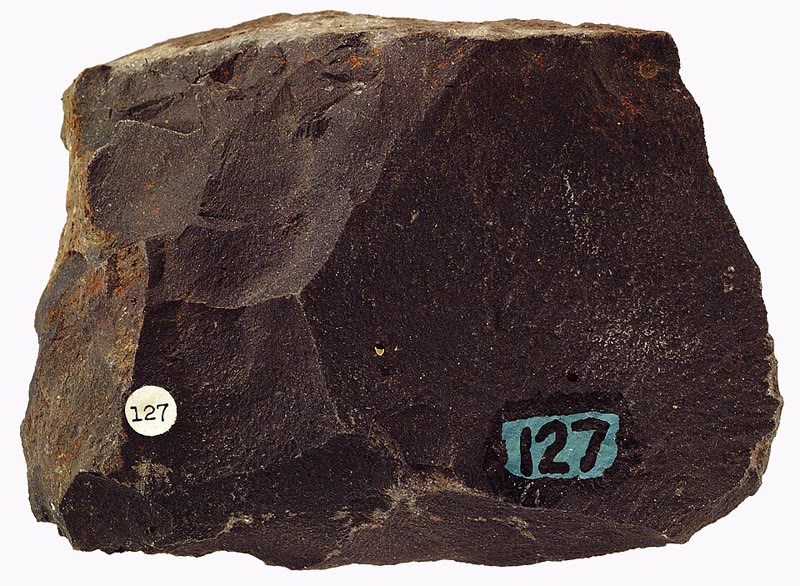
\includegraphics[height=2.9cm]{images/book2/g11-geodil-basalt.jpg}}\hfill
\makebox[0.32\linewidth]{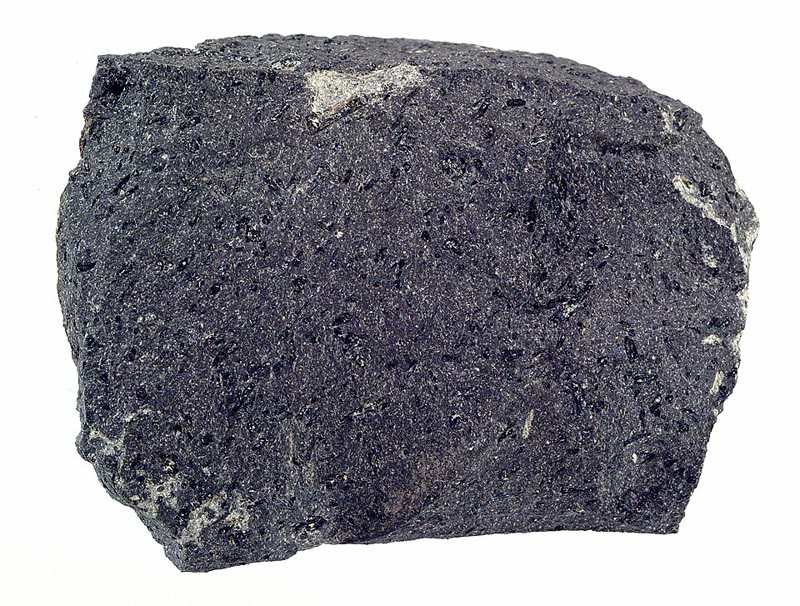
\includegraphics[height=2.9cm]{images/book2/g11-geodil-andesite.jpg}}\hfill
\makebox[0.32\linewidth]{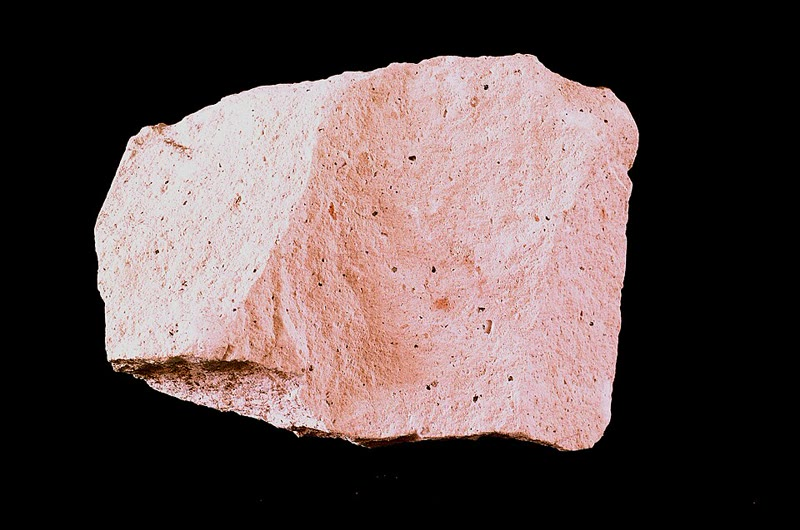
\includegraphics[height=2.9cm]{images/book2/g11-geodil-rhyolite.jpg}}

\smallskip
\makebox[0.32\linewidth]{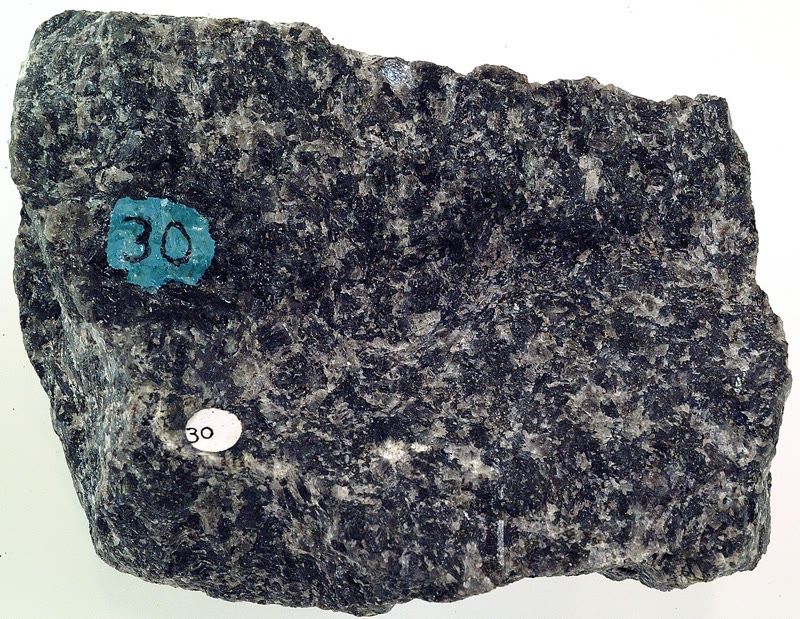
\includegraphics[height=2.9cm]{images/book2/g11-geodil-gabbro.jpg}}\hfill
\makebox[0.32\linewidth]{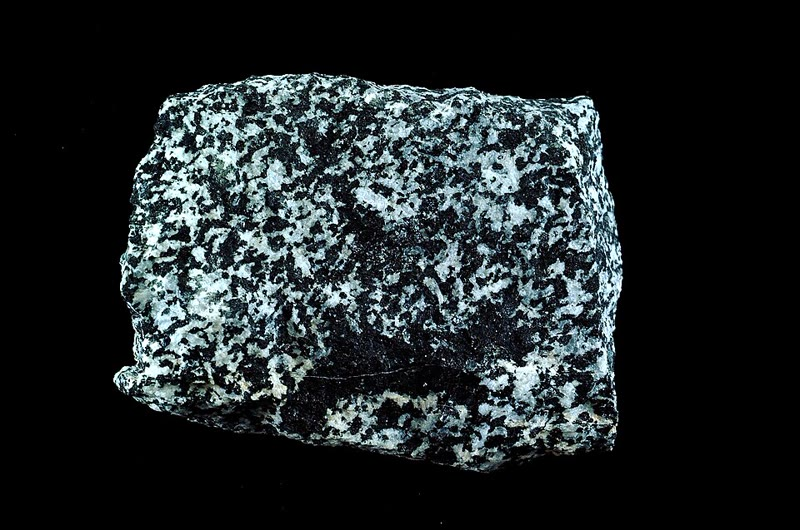
\includegraphics[height=2.9cm]{images/book2/g11-geodil-diorite.jpg}}\hfill
\makebox[0.32\linewidth]{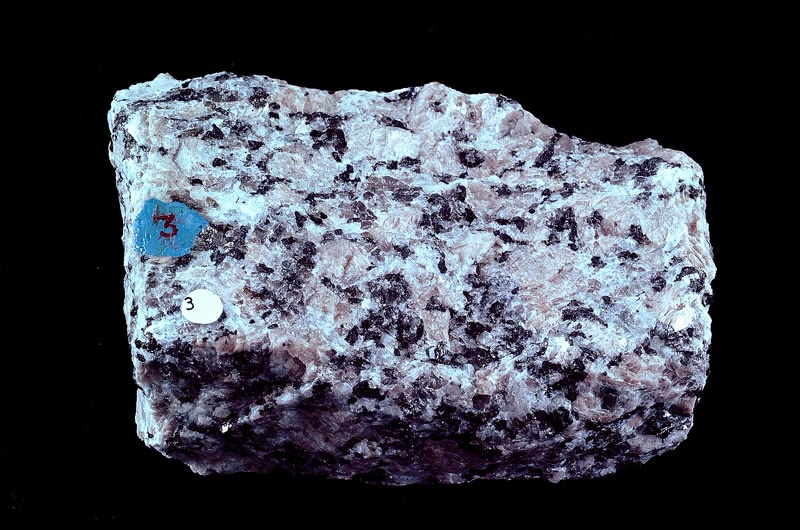
\includegraphics[height=2.9cm]{images/book2/g11-geodil-granite.jpg}}

{\small Les trois paires de roches magmatiques, de \omterm{def:g11:igneous-rocks:felsic-mafic}{mafique} à \omterm{def:g11:igneous-rocks:felsic-mafic}{felsique} de
gauche à droite~: \omterm{def:g11:igneous-rocks:volcanic-plutonic}{volcaniques} en haut, \omterm{def:g11:igneous-rocks:volcanic-plutonic}{plutoniques} en bas. En haut~: un
basalte à grain fin~; une \omterm{def:g11:igneous-rocks:rock-names}{andésite}, de petits cristaux d'amphibole dans une
pâte à grain fin (environ \qty{10}{cm})~; une \omterm{def:g11:igneous-rocks:rock-names}{rhyolite} rose. En bas~: un
\omterm{def:g11:ocean-ridges:gabbro}{gabbro} (\qty{9}{cm})~; une \omterm{def:g11:igneous-rocks:rock-names}{diorite}, hornblende noire et plagioclase vitreux
(\qty{10}{cm})~; un granite à gros grains avec de grands feldspaths
potassiques rose pâle, du plagioclase gris, du quartz, de la biotite et de
la hornblende (\qty{10}{cm}). Photographies Nessa Eull, Twyla Baker,
Joseph H.~Hartman, Darla Sondrol et Dexter Perkins, Geology Digital Image
Library (CC0).}
\end{omfigure}
% ledger: photo:g11-basalt, photo:g11-andesite, photo:g11-rhyolite, photo:g11-gabbro, photo:g11-diorite, photo:g11-granite

\section{L'ordre de cristallisation}

Un magma ne se fige pas à une seule température, comme l'eau. Ses minéraux
apparaissent les uns après les autres à mesure qu'il refroidit, chacun dans
son propre intervalle de température, si bien qu'un magma qui refroidit
peut contenir des cristaux tout en restant surtout liquide.

\begin{history}[Les expériences de Bowen]
Norman L.~Bowen (1887--1956) entra au Geophysical Laboratory de la Carnegie
Institution, à Washington, en 1912. Travaillant surtout sur des magmas
basaltiques, il faisait fondre une roche dans un four, la laissait
refroidir lentement jusqu'à une température choisie pour que certains
minéraux se forment, puis la trempait, en la refroidissant si vite que le
liquide restant devenait un verre. Au microscope, les cristaux montraient
quels minéraux s'étaient formés au-dessus de cette température. Répétée à
des températures de plus en plus basses, l'expérience donnait l'ordre
d'apparition des minéraux. Bowen publia cet ordre sous forme d'une série
réactionnelle en 1922, et son livre \emph{The Evolution of the Igneous
Rocks} en 1928.
\end{history}
% ledger: carnegie:bowen, earle:bowen

\begin{omfigure}
\begin{tikzpicture}[font=\footnotesize, box/.style={draw=black!60, rounded corners=2pt, fill=#1, minimum width=3.0cm, minimum height=0.62cm, align=center}]
  \node[box=omLithBasalt!45] (ol) at (0,0) {olivine};
  \node[box=omLithBasalt!35] (px) at (0,-1.1) {pyroxène};
  \node[box=black!15] (am) at (0,-2.2) {amphibole};
  \node[box=black!25] (bi) at (0,-3.3) {biotite};
  \draw[-{Stealth[length=4pt]}, line width=0.8pt] (ol) -- (px);
  \draw[-{Stealth[length=4pt]}, line width=0.8pt] (px) -- (am);
  \draw[-{Stealth[length=4pt]}, line width=0.8pt] (am) -- (bi);
  \node[align=center, anchor=south] at (0,0.45) {\textbf{branche discontinue}\\chaque minéral réagit avec\\le liquide pour donner le suivant};
  % continuous branch: a wedge from Ca-rich to Na-rich
  \fill[left color=omDef!55, right color=omDef!12, shading angle=180] (5.0,-0.9) -- (6.6,-0.9) -- (6.6,-3.5) -- (5.0,-3.5) -- cycle;
  \shade[top color=omDef!60, bottom color=omDef!10, draw=black!60, rounded corners=2pt] (4.3,-0.85) rectangle (7.3,-3.55);
  \node[align=center] at (5.8,-1.3) {plagioclase\\riche en calcium};
  \node[align=center] at (5.8,-3.15) {plagioclase\\riche en sodium};
  \draw[-{Stealth[length=4pt]}, line width=0.8pt] (5.8,-1.65) -- (5.8,-2.7);
  \node[align=center, anchor=south] at (5.8,0.45) {\textbf{branche continue}\\le plagioclase change\\progressivement};
  % last minerals
  \node[box=omLithGranite!45, minimum width=7.6cm] (last) at (2.9,-4.75) {feldspath potassique, quartz, (muscovite)};
  \draw[-{Stealth[length=4pt]}, line width=0.8pt] (bi) -- (bi |- last.north);
  \draw[-{Stealth[length=4pt]}, line width=0.8pt] (5.8,-3.55) -- (5.8,-4.43);
  % temperature arrow
  \draw[-{Stealth[length=5pt]}, line width=1pt, omThm] (-2.6,0.3) -- (-2.6,-4.9);
  \node[anchor=east, align=right, text=omThm] at (-2.75,0.1) {en premier,\\\qtyrange{1200}{1300}{\degreeCelsius}};
  \node[anchor=east, align=right, text=omThm] at (-2.75,-4.7) {en dernier, vers\\\qtyrange{750}{800}{\degreeCelsius}};
  \node[anchor=east, align=right, text=omThm] at (-2.75,-2.3) {température\\décroissante};
\end{tikzpicture}

{\small L'ordre dans lequel les minéraux cristallisent dans un magma qui
refroidit (la série réactionnelle de Bowen, schéma). L'olivine se forme en
premier~; le plagioclase commence à peu près en même temps que le pyroxène,
d'abord riche en calcium, puis de plus en plus riche en sodium. Le feldspath
potassique, le quartz et parfois la muscovite se forment en dernier, à
partir de ce qui reste d'un liquide riche en silice.}
\end{omfigure}
% ledger: earle:bowen

Le mot \emph{réactionnelle} compte. L'olivine n'est stable qu'à haute
température~: à mesure que le magma refroidit, les cristaux d'olivine
réagissent avec la silice du liquide et se transforment en pyroxène,
\[
  \ce{Mg2SiO4 + SiO2 -> 2 MgSiO3},
\]
et ainsi de suite le long de la branche, tant qu'il reste de la silice dans
le liquide. Le long de l'autre branche, les cristaux de plagioclase
continuent de grandir, mais chaque nouvelle couche est plus riche en sodium
que la précédente~: un cristal de plagioclase peut être zoné, d'un cœur
riche en calcium à une bordure riche en sodium, comme les \omterm{def:g11:igneous-rocks:porphyritic}{phénocristaux} de
plagioclase de l'\omterm{def:g11:igneous-rocks:rock-names}{andésite} ci-dessus.
% ledger: earle:bowen, photo:g11-andesite-xpl

La série explique le diagramme. Un magma \omterm{def:g11:igneous-rocks:felsic-mafic}{mafique} manque tôt de silice~: il
cristallise de l'olivine, du pyroxène et un plagioclase riche en calcium, et
donne un \omterm{def:g11:ocean-ridges:gabbro}{gabbro} s'il refroidit lentement sous terre, un basalte s'il
refroidit vite en surface. Seul un magma riche en silice va jusqu'au bout de
la série et forme du feldspath potassique et du quartz~: les minéraux du
granite et de la \omterm{def:g11:igneous-rocks:rock-names}{rhyolite}. La façon dont un magma change de composition en
chemin, quand ses premiers cristaux sont séparés du liquide, est l'objet de
la deuxième année d'université.
% ledger: earle:bowen, tulane:bowen

\section{Les intrusions}

Le magma monte parce qu'il est moins dense que les roches qui l'entourent,
en se frayant un chemin dans les fractures et en les élargissant. Une
grande partie n'atteint jamais la surface~: il cristallise dans la croûte
sous forme d'\omterm{def:g11:igneous-rocks:intrusion}{intrusions}, que l'on ne voit qu'une fois que l'érosion a
enlevé les roches qui les recouvraient.
% ledger: tulane:intrusions

\begin{definition}[Dyke~; sill~; pluton]\label{def:g11:igneous-rocks:intrusion}
Une \emph{intrusion}\index{intrusion} est un corps de roche magmatique qui a
cristallisé à l'intérieur d'autres roches. Un \emph{dyke}\index{dyke} (ou
filon) est une lame de roche magmatique qui recoupe les couches ou les
structures des roches qu'il traverse~; un \emph{sill}\index{sill} est une
lame parallèle aux couches, insérée entre elles. Un
\emph{pluton}\index{pluton} est une grande intrusion de forme quelconque,
formée en profondeur~; de nombreux plutons réunis forment un batholite
(\cref{ch:g12:subduction-magmatism}).
\end{definition}
% ledger: tulane:intrusions

Les \omterm{def:g11:igneous-rocks:intrusion}{dykes} ont en général moins de \qty{20}{m} de large et les \omterm{def:g11:igneous-rocks:intrusion}{sills} moins
de \qty{50}{m} d'épaisseur~; un \omterm{def:g11:igneous-rocks:intrusion}{sill} est d'ordinaire alimenté par un \omterm{def:g11:igneous-rocks:intrusion}{dyke}.
Les \omterm{def:g11:igneous-rocks:intrusion}{dykes} et les \omterm{def:g11:igneous-rocks:intrusion}{sills} peu profonds refroidissent vite~: ils sont à grain
fin, parfois \omterm{def:g11:igneous-rocks:porphyritic}{porphyriques}. Contre la roche froide qu'ils traversent, leurs
bords refroidissent plus vite encore et ont un grain plus fin que leur
centre~: c'est une \emph{bordure figée}, la marque d'un corps qui était
chaud quand il s'est mis en place. La Sierra Nevada de Californie, où se
trouve Yosemite, est un batholite~: les roches granitiques dont la masse
volumique a été mesurée au \cref{ch:g11:minerals} proviennent d'environ deux
cents de ses \omterm{def:g11:igneous-rocks:intrusion}{plutons}.
% ledger: tulane:intrusions, usgs91:sierra, photo:g11-el-capitan

\begin{omfigure}
\begin{tikzpicture}[font=\footnotesize, scale=0.9]
  % layered host rocks
  \fill[omLithSand] (0,0) rectangle (14,-1.0);
  \fill[omLithShale] (0,-1.0) rectangle (14,-2.0);
  \fill[omLithLime] (0,-2.0) rectangle (14,-3.0);
  \fill[omLithSand] (0,-3.0) rectangle (14,-4.0);
  \fill[omLithShale] (0,-4.0) rectangle (14,-6.4);
  \foreach \y in {-1,-2,-3,-4} \draw[black!35] (0,\y) -- (14,\y);
  % pluton
  \fill[omLithGranite, draw=black!60] (2.2,-6.4) .. controls (2.4,-4.6) and (3.6,-4.1) .. (5.5,-4.15)
     .. controls (7.4,-4.2) and (9.0,-4.5) .. (9.6,-6.4) -- cycle;
  % sill between the limestone and the shale, fed by the dyke
  \fill[omLithBasalt, draw=black!60] (7.3,-1.88) -- (12.6,-1.88) .. controls (12.9,-1.9) and (12.9,-2.1) .. (12.6,-2.12) -- (7.3,-2.12) -- cycle;
  % dyke from the pluton to the volcano
  \fill[omLithBasalt, draw=black!60] (7.0,-4.18) -- (7.3,-4.2) -- (7.3,0) -- (7.0,0) -- cycle;
  % a second dyke cutting across the layers, not reaching the surface
  \fill[omLithBasalt, draw=black!60] (3.9,-4.15) -- (4.15,-4.15) -- (2.95,-0.6) -- (2.75,-0.6) -- cycle;
  % volcano and lava flow
  \fill[black!65] (5.75,0) -- (7.15,1.35) -- (8.55,0) -- cycle;
  \fill[omLithBasalt!80!black] (8.4,0) -- (11.6,0) -- (11.6,0.1) .. controls (10.5,0.16) and (9.2,0.22) .. (8.3,0.15) -- cycle;
  \draw[black!70] (0,0) -- (5.75,0); \draw[black!70] (8.55,0) -- (14,0);
  % labels
  \node[anchor=south] at (7.15,1.4) {volcan};
  \draw[black!60] (10.5,0.15) -- (11.2,0.8); \node[anchor=south west, inner sep=1pt] at (11.2,0.8) {coulée de lave};
  \draw[black!60] (7.3,-0.5) -- (8.3,-0.5); \node[anchor=west, fill=omLithSand, inner sep=1pt] at (8.3,-0.5) {dyke (recoupe les couches)};
  \draw[black!60] (11.0,-2.0) -- (11.0,-2.55); \node[anchor=north, fill=omLithLime, inner sep=1pt] at (11.0,-2.55) {sill (entre les couches)};
  \draw[black!60] (3.4,-2.5) -- (1.9,-2.5); \node[anchor=east, fill=omLithLime, inner sep=1pt] at (1.9,-2.5) {dyke};
  \node[align=center] at (5.9,-5.5) {pluton};
  \node[anchor=east, fill=omLithShale, inner sep=1pt] at (13.85,-5.3) {roches sédimentaires litées};
\end{tikzpicture}

{\small Les \omterm{def:g11:igneous-rocks:intrusion}{intrusions} (schéma, sans échelle). Un \omterm{def:g11:igneous-rocks:intrusion}{pluton} cristallise en
profondeur~; des \omterm{def:g11:igneous-rocks:intrusion}{dykes} recoupent les couches des roches situées au-dessus,
l'un d'eux alimentant un volcan~; un \omterm{def:g11:igneous-rocks:intrusion}{sill} s'étale entre deux couches. Seule
l'érosion des roches qui les recouvrent met ces corps à nu en surface.}
\end{omfigure}
% ledger: tulane:intrusions

Combien de temps une \omterm{def:g11:igneous-rocks:intrusion}{intrusion} met-elle à cristalliser~? Considérons une
lame de magma --- un \omterm{def:g11:igneous-rocks:intrusion}{dyke} ou un \omterm{def:g11:igneous-rocks:intrusion}{sill} --- d'épaisseur $b$, qui perd sa
chaleur par conduction dans la roche des deux côtés. Les seules grandeurs
qui fixent le rythme sont l'épaisseur $b$, en mètres, et la diffusivité
thermique $\kappa$, en \unit{m^2/s}~; la seule durée que l'on puisse
construire avec elles est $b^2/\kappa$.
% ledger: england:kelvin, delaney86:example

\begin{proposition}[La durée de refroidissement d'une lame de magma]\label{prop:g11:igneous-rocks:cooling}
Une lame de magma d'épaisseur $b$ qui refroidit par conduction se solidifie
en un temps
\[
  t = C\,\frac{b^2}{\kappa},
\]
où $\kappa$ est la diffusivité thermique des roches et $C$ un nombre fixé
par les températures du magma et de la roche encaissante et par la chaleur
libérée par le magma en cristallisant. Doubler l'épaisseur multiplie la
durée par quatre. (Admis~; la valeur de $C$ provient d'un modèle calculé.)
\end{proposition}
% ledger: delaney86:properties, delaney86:example

Pour un magma basaltique injecté à \qty{1150}{\degreeCelsius} dans une
roche à \qty{50}{\degreeCelsius}, qui cristallise complètement à
\qty{950}{\degreeCelsius} et libère \qty{900}{MJ} de chaleur par mètre cube
cristallisé, avec $\kappa = \qty{1e-6}{m^2/s}$, le modèle donne
$C \approx 0.21$. Une lame épaisse de \qty{2}{m} se solidifie alors en une
dizaine de jours, un \omterm{def:g11:igneous-rocks:intrusion}{sill} épais de \qty{20}{m} en deux ans et demi environ,
un \omterm{def:g11:igneous-rocks:intrusion}{sill} de \qty{100}{m} en soixante-cinq ans environ. Sans la
chaleur de cristallisation, les durées seraient trois fois plus courtes~:
le magma qui cristallise se maintient lui-même au chaud.
% values (dyke_cooling.py): t2_day 9.55, t20_yr 2.61, t100_yr 65.3, latent_factor 2.94; C = 8.2475e7 s / 4e8 s = 0.206
% ledger: delaney86:example, delaney86:properties, england:kelvin

\begin{omfigure}
\begin{tikzpicture}
\begin{axis}[omrecord, name=times, width=0.45\linewidth, height=5.0cm, xmode=log, ymode=log,
  xmin=0.8, xmax=130, ymin=1e-3, ymax=200, xlabel={épaisseur de la lame (\unit{m})},
  ylabel={durée de solidification (années)},
  legend style={font=\scriptsize, at={(0.5,-0.4)}, anchor=north, legend columns=2,
    /tikz/every even column/.append style={column sep=4pt}}]
% computed in figdata/grade-11/dyke_cooling.py; ledger: delaney86:*, england:kelvin
\addplot[omThm, line width=1pt, mark=*, mark size=1.4pt] table[x=b, y=t_yr] {figdata/out/grade-11-dyke_cooling-times.dat};
\addplot[omDef, line width=1pt, dashed, mark=o, mark size=1.4pt] table[x=b, y=t0_yr] {figdata/out/grade-11-dyke_cooling-times.dat};
\legend{avec la chaleur de cristallisation, sans}
\end{axis}
\begin{axis}[omrecord, at={(times.east)}, anchor=west, xshift=1.6cm, width=0.45\linewidth, height=5.0cm,
  xmin=-28, xmax=28, ymin=0, ymax=1300, xlabel={distance au centre du sill (\unit{m})},
  ylabel={température (\unit{\degreeCelsius})},
  legend style={font=\scriptsize, at={(0.5,-0.4)}, anchor=north, legend columns=4,
    /tikz/every even column/.append style={column sep=4pt}}]
\fill[omLithBasalt!30] (axis cs:-10,0) rectangle (axis cs:10,1300);
\draw[black!50, dashed] (axis cs:-28,950) -- (axis cs:28,950);
\node[font=\scriptsize, anchor=south east, text=black!60] at (axis cs:27,955) {solidus};
\node[font=\scriptsize, anchor=north] at (axis cs:0,1290) {sill};
% computed in figdata/grade-11/dyke_cooling.py
\addplot[omProp, line width=0.9pt] table[x=x, y=T1] {figdata/out/grade-11-dyke_cooling-profiles.dat};
\addplot[omThm, line width=0.9pt] table[x=x, y=T2] {figdata/out/grade-11-dyke_cooling-profiles.dat};
\addplot[omDef, line width=0.9pt] table[x=x, y=T3] {figdata/out/grade-11-dyke_cooling-profiles.dat};
\addplot[black, line width=0.9pt] table[x=x, y=T4] {figdata/out/grade-11-dyke_cooling-profiles.dat};
\legend{30 jours, 6 mois, 1 an, 2 ans}
\end{axis}
\end{tikzpicture}

{\small Une lame de magma basaltique qui refroidit par conduction (modèle
calculé). À gauche~: la durée de solidification en fonction de
l'épaisseur, sur des axes logarithmiques~: une droite de pente 2, la durée
croissant comme le carré de l'épaisseur. À droite~: les températures à
travers un \omterm{def:g11:igneous-rocks:intrusion}{sill} épais de \qty{20}{m} (en grisé), injecté à
\qty{1150}{\degreeCelsius} dans une roche à \qty{50}{\degreeCelsius}. Les
bords passent aussitôt sous le solidus, le centre seulement au bout de deux
ans et demi environ.}
\end{omfigure}
% values (dyke_cooling.py): profiles at 30, 180, 365, 730 days; contact about 690 degC (Delaney: 690)

Le modèle montre aussi la formation de la bordure figée. La roche au contact
passe aussitôt à environ \qty{690}{\degreeCelsius}, bien en dessous du
solidus~: les premiers centimètres du \omterm{def:g11:igneous-rocks:intrusion}{sill} se figent en moins d'un jour,
alors que son centre reste liquide pendant des années. Les \omterm{def:g11:igneous-rocks:intrusion}{intrusions}
réelles sont plus compliquées --- les propriétés des roches changent avec
la température, l'eau circule, un \omterm{def:g11:igneous-rocks:intrusion}{pluton} profond se trouve dans une roche
déjà chaude et peut être alimenté encore et encore ---, ce qui explique que
les grandes \omterm{def:g11:igneous-rocks:intrusion}{intrusions} profondes mettent bien plus longtemps à refroidir que
ne le suggérerait la loi, avec un encaissant froid.
% ledger: delaney86:example, tulane:cooling-times
% values (dyke_cooling.py): margin_day_20m 0.58 (cell 12.5 cm from the contact)

\section{Exercices}

\begin{exercise}[$\star$]\label{exo:g11:igneous-rocks:1}
Définir une \omterm{def:g11:igneous-rocks:volcanic-plutonic}{roche volcanique} et une \omterm{def:g11:igneous-rocks:volcanic-plutonic}{roche plutonique}. Donner les trois
paires de \omterm{def:g11:igneous-rocks:volcanic-plutonic}{roches volcaniques} et \omterm{def:g11:igneous-rocks:volcanic-plutonic}{plutoniques} de même composition, de la plus
\omterm{def:g11:igneous-rocks:felsic-mafic}{mafique} à la plus \omterm{def:g11:igneous-rocks:felsic-mafic}{felsique}.
\end{exercise}

\begin{exercise}[$\star$]\label{exo:g11:igneous-rocks:2}
Associer chaque roche à sa \omterm{def:g11:igneous-rocks:texture}{texture} --- vitreuse, à grain fin, à gros
grains, \omterm{def:g11:igneous-rocks:porphyritic}{porphyrique}~: (1) l'obsidienne~; (2) le granite~; (3) un basalte
contenant des cristaux verts d'olivine de quelques millimètres dans une pâte
sombre~; (4) un basalte dans lequel aucun minéral n'est visible.
\end{exercise}

\begin{exercise}[$\star$]\label{exo:g11:igneous-rocks:3}
Trois magmas contiennent \qty{48}{\percent}, \qty{60}{\percent} et
\qty{72}{\percent} de \ce{SiO2}. Classer chacun, et nommer la roche que
chacun donne quand il refroidit lentement en profondeur.
\end{exercise}

\begin{exercise}[$\star$]\label{exo:g11:igneous-rocks:4}
Définir un \omterm{def:g11:igneous-rocks:intrusion}{dyke}, un \omterm{def:g11:igneous-rocks:intrusion}{sill} et un \omterm{def:g11:igneous-rocks:intrusion}{pluton}. Sur le schéma des \omterm{def:g11:igneous-rocks:intrusion}{intrusions} de ce
chapitre, quel corps a alimenté le volcan~?
\end{exercise}

\begin{exercise}[$\star$]\label{exo:g11:igneous-rocks:5}
Dans la série réactionnelle de Bowen, quel minéral se forme en premier, et
quels minéraux se forment en dernier~? Comment le plagioclase change-t-il
à mesure que le magma refroidit~?
\end{exercise}

\begin{exercise}[$\star\star$]\label{exo:g11:igneous-rocks:6}
On analyse deux roches (pourcentages en masse). Roche A~: \ce{SiO2} 74,
\ce{Al2O3} 14, \ce{FeO} 3, \ce{CaO} 3, \ce{MgO} 0.5, \ce{Na2O} 5, \ce{K2O} 4.
Roche B~:
\ce{SiO2} 47, \ce{Al2O3} 14, \ce{FeO} 8, \ce{CaO} 10, \ce{MgO} 8, \ce{Na2O}
1, \ce{K2O} 2. (1) Classer chacune. (2) Vérifier la réponse avec les autres
oxydes. (3) La roche A est à grain fin~: la nommer. La roche B est à gros
grains~: la nommer.
\end{exercise}

\begin{exercise}[$\star\star$]\label{exo:g11:igneous-rocks:7}
Un \omterm{def:g11:igneous-rocks:intrusion}{dyke} épais de \qty{2}{m} se solidifie en une dizaine de jours. À l'aide
de la proposition sur la durée de refroidissement, combien de temps met un
\omterm{def:g11:igneous-rocks:intrusion}{dyke} du même magma s'il est épais de \qty{1}{m}~? Un \omterm{def:g11:igneous-rocks:intrusion}{sill} épais de
\qty{20}{m}~? Un \omterm{def:g11:igneous-rocks:intrusion}{sill} épais de \qty{200}{m}~?
\end{exercise}

\begin{exercise}[$\star\star$]\label{exo:g11:igneous-rocks:8}
(1) Montrer que $b^2/\kappa$ est une durée. (2) La calculer pour
$b = \qty{20}{m}$ et $\kappa = \qty{1e-6}{m^2/s}$, en secondes et en années
($\num{1}\text{ an} \approx \qty{3.16e7}{s}$). (3) Avec $C = 0.21$,
combien de temps le \omterm{def:g11:igneous-rocks:intrusion}{sill} met-il à se solidifier~?
\end{exercise}

\begin{exercise}[$\star\star$]\label{exo:g11:igneous-rocks:9}
Une roche montre des cristaux trapus de plagioclase longs d'environ un
centimètre dans une pâte dont on ne voit pas les grains. Décrire sa
\omterm{def:g11:igneous-rocks:texture}{texture}, et raconter l'histoire de son refroidissement en deux étapes.
\end{exercise}

\begin{exercise}[$\star\star$]\label{exo:g11:igneous-rocks:10}
L'olivine réagit avec la silice du liquide~: $\ce{Mg2SiO4 + SiO2 -> 2
MgSiO3}$. (1) Vérifier que l'équation est équilibrée. (2) Avec les masses
molaires \qty{140.7}{g/mol} (\ce{Mg2SiO4}) et \qty{60.1}{g/mol}
(\ce{SiO2}), quelle masse de silice \qty{1}{kg} d'olivine prend-il au
liquide~? (3) Pourquoi un magma pauvre en silice garde-t-il son olivine~?
\end{exercise}

\begin{exercise}[$\star\star$]\label{exo:g11:igneous-rocks:11}
Un \omterm{def:g11:igneous-rocks:intrusion}{sill} épais de \qty{20}{m} et d'une surface de \qty{1}{m^2} refroidit de
\qty{1150}{\degreeCelsius} à \qty{50}{\degreeCelsius}. (1) Sa capacité
thermique est de \qty{2.5}{MJ} par mètre cube et par degré~: quelle chaleur
perd-il en refroidissant~? (2) Il libère aussi \qty{900}{MJ} par mètre cube
en cristallisant~: quelle chaleur cela représente-t-il~? (3) Comparer les
deux.
\end{exercise}

\begin{exercise}[$\star\star\star$]\label{exo:g11:igneous-rocks:12}
Dans le modèle calculé d'un \omterm{def:g11:igneous-rocks:intrusion}{sill} épais de \qty{20}{m}, la roche située à
\qty{12.5}{cm} du contact passe sous le solidus au bout d'environ
\num{0.6}~jour, la roche située à \qty{5}{m} du contact au bout d'environ
545 jours, et le centre au bout d'environ 950 jours. (1) Où, dans le \omterm{def:g11:igneous-rocks:intrusion}{sill},
s'attend-on à trouver les plus petits cristaux, et où les plus grands~?
(2) La vitesse à laquelle la couche solide s'épaissit est-elle constante~?
(3) Pourquoi le \omterm{def:g11:igneous-rocks:intrusion}{sill} est-il à grain fin même en son centre, comparé à un
granite~?
\end{exercise}

\begin{exercise}[$\star\star\star$]\label{exo:g11:igneous-rocks:13}
Un \omterm{def:g11:igneous-rocks:intrusion}{pluton} est épais de \qty{2}{km}. (1) À l'aide de la proposition et du
\omterm{def:g11:igneous-rocks:intrusion}{sill} de \qty{20}{m} (environ 2.6 ans), estimer sa durée de refroidissement.
(2) On sait que les grandes \omterm{def:g11:igneous-rocks:intrusion}{intrusions} profondes mettent jusqu'à des
millions d'années à refroidir. Donner deux raisons pour lesquelles la loi
simple sous-estime la durée.
\end{exercise}

\begin{exercise}[$\star\star\star$]\label{exo:g11:igneous-rocks:14}
Les magmas \omterm{def:g11:igneous-rocks:felsic-mafic}{felsiques} font éruption vers
\qtyrange{650}{800}{\degreeCelsius}, les magmas \omterm{def:g11:igneous-rocks:felsic-mafic}{mafiques} vers
\qtyrange{1000}{1200}{\degreeCelsius}. À l'aide de la série réactionnelle
de Bowen, expliquer pourquoi un granite contient du feldspath potassique,
du quartz et un plagioclase riche en sodium, et pas d'olivine, alors qu'un
\omterm{def:g11:ocean-ridges:gabbro}{gabbro} contient de l'olivine, du pyroxène et un plagioclase riche en
calcium, et pas de quartz.
\end{exercise}

\begin{exercise}[$\star\star\star$]\label{exo:g11:igneous-rocks:15}
Les matériaux projetés dans l'air refroidissent en quelques secondes, les
coulées de lave en quelques jours à quelques semaines, les \omterm{def:g11:igneous-rocks:intrusion}{intrusions} peu
profondes en quelques mois à quelques années. (1) À l'aide de la
proposition, quelle épaisseur de lame se solidifie en un jour environ~?
(2) Une coulée de lave épaisse de \qty{5}{m} se solidifie en un mois
environ~: est-ce cohérent avec la loi pour une lame refroidie des deux
côtés~? (3) Quelle \omterm{def:g11:igneous-rocks:texture}{texture} attend-on dans chaque cas~?
\end{exercise}

\section{Problème~: un sill et ses cristaux}

\begin{problem}[{Problème du week-end --- combien de temps un sill met à se figer}]
\label{pb:g11:igneous-rocks:1}
% values (dyke_cooling.py): t20_yr 2.61, margin_day_20m 0.58, t2_day 9.55, contact ~690 degC;
% C = 0.206; ledger delaney86:*, tulane:*, earle:*
Dans la paroi d'une vallée, une lame sombre de roche magmatique épaisse de
\qty{20}{m} s'intercale entre deux bancs de grès, parallèlement à eux. On
prélève des échantillons de son bord jusqu'à son centre. Au contact, la
roche est à grain très fin, presque vitreuse~; à \qty{1}{m} à l'intérieur,
ses cristaux mesurent environ \qty{0.1}{mm}~; au centre, environ
\qty{1}{mm}, et on distingue tout juste le plagioclase et le pyroxène à la
loupe.

\medskip
\noindent\textbf{Partie I --- Les textures.}
\begin{enumerate}
  \item La lame est-elle un \omterm{def:g11:igneous-rocks:intrusion}{dyke} ou un \omterm{def:g11:igneous-rocks:intrusion}{sill}~? Pourquoi~?
  \item Décrire la \omterm{def:g11:igneous-rocks:texture}{texture} au contact et au centre.
  \item Pourquoi la roche a-t-elle le grain le plus fin au contact~?
  \item Comment s'appelle cette bordure à grain fin, et que prouve-t-elle
        sur la température de la lame au moment de sa mise en place~?
  \item La lame est alimentée par le bas par une lame verticale de la même
        roche, épaisse de \qty{2}{m}, qui recoupe le grès. De quoi
        s'agit-il~?
\end{enumerate}

\medskip
\noindent\textbf{Partie II --- Nommer la roche.}
\begin{enumerate}[resume]
  \item Une analyse donne \qty{49}{\percent} de \ce{SiO2},
        \qty{10}{\percent} de \ce{FeO}, \qty{7}{\percent} de \ce{MgO} et
        \qty{10}{\percent} de \ce{CaO}. Le magma est-il \omterm{def:g11:igneous-rocks:felsic-mafic}{mafique},
        \omterm{def:g11:igneous-rocks:felsic-mafic}{intermédiaire} ou \omterm{def:g11:igneous-rocks:felsic-mafic}{felsique}~?
  \item Quels minéraux attend-on, d'après la série de Bowen~?
  \item Quel nom convient à la roche du contact~? Quelle \omterm{def:g11:igneous-rocks:volcanic-plutonic}{roche plutonique} a
        la même composition~?
  \item Pourquoi un même corps de magma peut-il donner des roches de
        \omterm{def:g11:igneous-rocks:texture}{textures} différentes~?
  \item Dans quel ordre l'olivine, le pyroxène et le plagioclase ont-ils
        commencé à cristalliser~?
\end{enumerate}

\medskip
\noindent\textbf{Partie III --- La durée de refroidissement.}
\begin{enumerate}[resume]
  \item Calculer $b^2/\kappa$ pour le \omterm{def:g11:igneous-rocks:intrusion}{sill}, avec
        $\kappa = \qty{1e-6}{m^2/s}$, en secondes.
  \item Le modèle donne $C = 0.206$. Calculer la durée de solidification
        du \omterm{def:g11:igneous-rocks:intrusion}{sill}, en secondes, puis en années
        ($\num{1}\text{ an} \approx \qty{3.16e7}{s}$).
  \item Combien de temps a mis la lame d'alimentation, épaisse de
        \qty{2}{m}~?
  \item Sans la chaleur de cristallisation, $C$ vaudrait environ $0.07$.
        Combien de temps mettrait le \omterm{def:g11:igneous-rocks:intrusion}{sill}~? Pourquoi la cristallisation
        ralentit-elle le refroidissement~?
  \item Le modèle donne environ \num{0.6}~jour pour la roche située à
        \qty{12.5}{cm} du contact. Combien de fois plus vite s'est-elle
        figée que le centre~?
\end{enumerate}

\medskip
\noindent\textbf{Partie IV --- Ce que disent les cristaux.}
\begin{enumerate}[resume]
  \item Les coulées de lave refroidissent en quelques jours à quelques
        semaines, les \omterm{def:g11:igneous-rocks:intrusion}{intrusions} peu profondes en quelques mois à quelques
        années. Où se place le \omterm{def:g11:igneous-rocks:intrusion}{sill}~?
  \item Un granite aux cristaux d'un centimètre ou plus a refroidi bien
        plus lentement. Estimer, à l'aide de la loi, l'épaisseur d'une lame
        qui mettrait mille fois plus de temps que le \omterm{def:g11:igneous-rocks:intrusion}{sill}.
  \item Pourquoi un tel corps a-t-il dû se former en profondeur dans la
        croûte~?
  \item Le \omterm{def:g11:igneous-rocks:intrusion}{sill} est visible aujourd'hui en surface. Qu'a-t-il dû arriver
        aux roches qui le recouvraient~?
  \item Conclure~: combien de temps le \omterm{def:g11:igneous-rocks:intrusion}{sill} a-t-il mis à se solidifier~?
\end{enumerate}
\end{problem}
